\documentclass[letterpaper,12pt]{article}
\usepackage[T1]{fontenc}
\usepackage{mathptmx}

% unit definition
\usepackage{siunitx}
% \sisetup{load-configurations = abbreviations}
\DeclareSIUnit\inch{in}
\DeclareSIUnit\ft{ft}
\DeclareSIUnit\Rank{^{\circ} R}
\DeclareSIUnit\Faren{^{\circ} F}
\DeclareSIUnit\lbm{lb_{m}}
\DeclareSIUnit\lbf{lb_{f}}
\DeclareSIUnit\torr{Torr}
\DeclareSIUnit\gallon{gal}
\DeclareSIUnit\slug{slug}
\DeclareSIUnit\knots{kts}
\DeclareSIUnit\miles{mi}


% hyperlink formatting
\usepackage{hyperref}
\hypersetup{
    colorlinks=true,
    linkcolor=red,
    urlcolor=purple,
    citecolor=blue
}


% Other general packages
\usepackage{setspace}
\usepackage{graphicx}
\usepackage{float}
\usepackage{amsmath}
\usepackage{amssymb}
\usepackage{tabto}
\usepackage{booktabs, tabularx}
\usepackage{enumitem}
\usepackage{gensymb}
\usepackage{cancel}
\usepackage{tikz}
\usepackage{pgfplots}
\usepackage{appendix}
\usepackage[labelfont=bf, font={normalsize,stretch=1}]{caption}
\usepackage[letterpaper, margin=1.0in]{geometry}
\usepackage[utf8]{}
\usepackage{indentfirst}
\setlength{\parindent}{0.25in}

%Heading format
\usepackage{titlesec}
\titleformat*{\section}{\normalsize\bfseries}
\titleformat*{\subsection}{\normalsize\bfseries}
\titleformat*{\subsubsection}{\normalsize\bfseries}

%Page Numbers
\usepackage{fancyhdr} 
\pagestyle{fancy}
\fancyhf{}
\fancyheadoffset{0cm}
\renewcommand{\headrulewidth}{0pt} 
\renewcommand{\footrulewidth}{0pt}
\fancyhead[R]{\thepage}
\pagenumbering{arabic}

%listings package for code
\usepackage{listings}
\usepackage{xcolor}

% bibliography formatting
\usepackage{etoolbox}
\patchcmd{\thebibliography}{\section*{\refname}}{}{}{}
\setstretch{2}

% color definitions
\definecolor{dblue}{HTML}{145680}
\definecolor{dred}{HTML}{801414}
\definecolor{dgreen}{HTML}{148014}
\definecolor{bgcode}{rgb}{0.95,0.95,0.95}
\definecolor{codegreen}{rgb}{0,0.6,0}
\definecolor{codegray}{rgb}{0.5,0.5,0.5}
\definecolor{codepurple}{rgb}{0.58,0,0.82}
\definecolor{backcolour}{rgb}{0.95,0.95,0.92}

\lstdefinestyle{mystyle}{
    backgroundcolor=\color{backcolour},
    commentstyle=\color{codegreen},
    keywordstyle=\color{magenta},
    numberstyle=\tiny\color{codegray},
    stringstyle=\color{codepurple},
    basicstyle=\ttfamily\footnotesize,
    breakatwhitespace=false,
    breaklines=true,
    captionpos=b,
    keepspaces=true,
    numbers=left,
    numbersep=5pt,
    showspaces=false,
    showstringspaces=false,
    showtabs=false,
    tabsize=2
}
\lstset{style=mystyle}

\pgfplotsset{compat=1.17}

% NOTES
%  - Double spacing (always fix for figures and tables though)
%  - for tables, remember to make them single spaced using \renewcommand{\arraystretch}{1}
%  - Always pull from GitHub to Overleaf when there are commits to be pulled (Menu > GitHub > PULL)
%  - for REFERENCES, use \cite{<label>} to link the reference.

% % TABLE TEMPLATE
% \begin{table}[H]
%     \begin{center}
%     \setstretch{1} 
%     \caption{\textbf{<caption here>}} \label{table:<label here>}
%     \begin{tabular}{|p{0.3in}|p{1in}|p{1in}|} % set column nums and width
%         \hline \textbf{No.} & \textbf{Item} & \textbf{Weight} \\ \hline % column headers
%         1 & Hot dogs & 2 lbs \\ \hline
%     \end{tabular}
%     \end{center}
% \end{table}

\begin{document}

%%% Title Pa
\begin{center}
    {\Large\textbf{AE 484 Homework 2}}\\
    Anshuk Chigullapalli, George Petrov, Kenneth Tochihara, Jeffery Zhou\\
\end{center}


\section{Group name and leader}
% Determine a group name and vote/select a group leader

    \textbf{Group Name:} Illinois Air Society % subject to change
    
    \textbf{Group Leader:} George Petrov % subject to change

\section{Existing tailless RC aircraft}
% Search the internet or publications and evaluate 4 flying wing (tailless) R/C or UAV aircraft. In a table determine the following: Name of the aircraft, Wing planform area, Winglet planform area, weight of the aircraft, wing loading (W/S), Wing sweep, Wing taper ratio, wing root chord length, wing tip chord length, wing span, motor position (tractor or pusher), motor size (power), link or reference where information was gathered. Note that many of these quantities are estimates and may need to be scaled from pictures or schematics.

    \begin{table}[H]
        \begin{tabular}{|c|c|c|c|c|} % set column nums and width
            \hline \textbf{Name} & \textbf{Wing area (in$^\textbf{2}$)} & \textbf{Winglet area (in$^\textbf{2}$)} & \textbf{Weight (lb)} & \textbf{Loading (oz/in$^2$)} \\ \hline % column headers
            RQ-170 & 40512.5 & 0 & 8500 & 3.36 \\ \hline
            Northrop Grumman Bat & 7125 & 351 & 350 & 0.786 \\ \hline
            Skynetic Neptune II Blue & 381.8 & 0 & 1.256 & 0.0526 \\ \hline
            Northrop Grumman X-47B & 137318.4 & 0 & 14000 & 5.127 \\ \hline
        \end{tabular}
    \end{table}
    
    \begin{table}[H]
        \begin{tabular}{|c|c|c|c|c|c| } % set column nums and width
            \hline \textbf{Name} & \textbf{Sweep} & \textbf{Taper ratio} & \textbf{Root chord (in)} & \textbf{Tip chord (in)} & \textbf{Span (in)} \\ \hline % column headers
            RQ-170 & 33$\degree$ & 0.187 & 148 & 27 & 463 \\ \hline
            Northrop Grumman Bat & 46$ \degree$ & 0.3 & 73 & 22 & 168 \\ \hline
            Skynetic Neptune II Blue & 33$ \degree$ & 0.481 & 13.12 & 6.310 & 39.3 \\ \hline
            Northrop Grumman X-47B & 70 $\degree$ & 0.67 & 456 & 305.52 & 744\\ \hline
        \end{tabular}
    \end{table}
    
    \begin{table}[H]
        \begin{tabular}{|c|c|c|c| } % set column nums and width
            \hline \textbf{Name} & \textbf{Motor position} & \textbf{Motor size} & \textbf{Reference} \\ \hline % column headers
            RQ-170  & Pusher & \href{https://en.wikipedia.org/wiki/General_Electric_TF34}{General Electric TF34} & \href{https://en.wikipedia.org/wiki/Lockheed_Martin_RQ-170_Sentinel}{Wikipedia}\\ \hline
            Northrop Grumman Bat & Pusher & Hirth Engine & \href{https://en.wikipedia.org/wiki/Northrop_Grumman_Bat}{Wikipedia}\\ \hline

             Skynetic Neptune II Blue & Pusher & ASS2212 KV (1.1" diameter) & \href{https://www.motionrc.com/products/skynetic-neptune-ii-blue-1000mm-39-3-wingspan-pnp?variant=39681690927289}{MotionRC}\\ \hline
             Northrop Grumman X-47B & Pusher & Pratt Whitney F100-220U & \href{https://www.militaryfactory.com/aircraft/detail.php?aircraft_id=1015}{MilitaryFactory} \\ \hline
        \end{tabular}
    \end{table}

\section{Objectives and Constraints}
% Write a paragraph summarizing objectives and what constraints are place on your design. In addition to the mission objectives create bulleted items of design objectives and constraints which your vehicle should meet with numerical values when possible. Mark each numbered bulleted item with a 1 thru 3 number indicating the level of importance (1-vehicle must meet item, 2-some flexibility in item, 3-optional).

    The overall objective of the mission is to design and build a mini-UAV that deploys a vial of vaccine to a remote area. This UAV shall be hand-launched and shall land without any landing gears. Testing shall remain within line-of-sight (LOS) and shall abide by the Academy of Model Aeronautics (AMA) guidelines. The UAV shall be tailless with only two control surfaces (one elevon on each wing). Propeller/Motor/Speed Controller/Battery combinations are provided and shall be utilized within the design. This UAV shall be capable of achieving altitude quickly. The UAV's wings shall be made with Balsa reinforced foam with a fiberglass covering and shall be propelled with a tractor or pusher configuration.
    The following points highlight the numerical constraints of the problem statement.
    
    \begin{itemize}
        \item \textbf{Max Altitude (1):} 400 ft
        \item \textbf{Flight Time (2):} 15 min
        \item \textbf{Top Speed (2):} 40 mph
        \item \textbf{Max Thickness (3):} 1.75 in
        \item \textbf{Max Wingspan (1):} 70 in
        \item \textbf{Max Weight (3):} 3 lbs
    \end{itemize}

\section{Individual Vehicle Concepts}
% Each individual in your group must present one vehicle concept. Each individual should present a three-view drawing (CAD preferred, but very nice ruler and template drawn sketches acceptable) and isometric view of their vehicle configuration the individual proposes with basic (overall) dimensions to ascertain the general size and shape. Indicate which individual is responsible for each design (points may be deducted from the overall grade for individuals who do not have a professional presentation of their concept).

    The engineering drawings of each individual member's CAD designs are attached at the end of the assignment.

\section{Weight and Wing Loading of Vehicle Concepts}
% Estimate the weight and wing loading of each concept aircraft (take-off weight). Be sure to include all instrumentation, cargo, battery, etc. in your analysis. Also indicate how you estimated the weight of the structure (i.e. fuselage, spars, skin, bulkheads, winglets, etc.) in the concept drawings. Be sure to include a table with all the weights of the components clearly presented and example calculations of estimated values
    
    \subsection{Anshuk}
    \begin{table}[H]
        \begin{tabular}{|c|c| } % set column nums and width
            \hline \textbf{Component} & \textbf{Mass (g)} \\ \hline % column headers
            \href{https://www.amazon.com/Brushless-Outrunner-Multicopters-Helicopter-Control/dp/B08MKQFSVF/ref=asc_df_B08MKQFSVF/?tag=hyprod-20&linkCode=df0&hvadid=475795164185&hvpos=&hvnetw=g&hvrand=9902342740412303481&hvpone=&hvptwo=&hvqmt=&hvdev=c&hvdvcmdl=&hvlocint=&hvlocphy=2840&hvtargid=pla-1195392311214&th=1}{GFORCE E480 BRUSHLESS OUTRUNNER MOTOR (3530 - 1100KV)} & 100 \\ \hline
            \href{http://www.valuehobby.com/gforce-40a-esc.html}{GFORCE 40A BRUSHLESS ESC (T-CONNECTOR)} & 35 \\ \hline
            \href{http://www.valuehobby.com/30c-2200mah-3s-t.html}{GFORCE 30C 2200MAH 3S 11.1V LIPO (T-CONNECTOR)} & 186 \\ \hline
            \href{https://www.masterairscrew.com/products/electric-only-12x6-propeller?currency=USD&utm_medium=cpc&utm_source=google&utm_campaign=Google\%20Shopping&gclid=CjwKCAiA9aKQBhBREiwAyGP5laqPgb8z2BGon5sD8qHYRZQVab7IcA0DZg8DOcFMsDTccBgRqirzgBoC1wkQAvD_BwE}{Electric Only - 12x6 Propeller} & 27 \\ \hline
            \href{https://www.horizonhobby.com/product/ar620-dsmx-6-channel-sport-receiver/SPMAR620.html?gclid=CjwKCAiA9aKQBhBREiwAyGP5lX6-hyQKl87DI0WH0pgWG2HS0woZKcd-L2bMRS_qWmVI1fLqpeCX0BoCrRAQAvD_BwE}{Spektrum AR620 DSMX 6-Channel Sport Receiver} & 8 \\ \hline
            \href{https://arrishobby.com/emax-es08ma-ii-12g-mini-metal-gear-analog-servo-p0842.html?VariantsId=12700}{EMAX ES08MA II ANALOG METAL GEAR MICRO SERVO} & 36 \\ \hline
            Wing & 560 \\ \hline
            Fuselage "bump" & 350 \\ \hline
            Vial & 5 \\ \hline
            \textbf{Total} & 1307 \\ \hline
        \end{tabular}
        \end{table}
        The weight estimates of the COTS components is based on the parts provided in the problem statement, such as the brush-less motor and the vial. Other COTS components, such as the micro-servo and the propeller, were obtained from providers online (references are hyperlinked in the table above). 
        
        For the weight of the wings themselves, the given wing area density of 0.033 oz/in$^2$ was used. The wing area of this design was 597.753 in$ ^2 $. With these values, we get the weight of the wing to be 19.73 oz $ = $ 560 grams.
        The aircraft has no winglets. There is also no explicit fuselage, however the fused "bump" that houses the vial and all electric components adds the additional weight of roughly 350 grams that includes the weight of the skin and any required supports. The aircraft also doesn't have a vertical stabilizer, and so no additional mass is added there.
        
        The total weight of the weight of the aircraft is approximated to be 1307 grams, or 2.88 lbs. Therefore, the design is currently under the weight limit. The wing loading based on the wing area and the calculating weight of the aircraft is 0.077 oz/in$^2$. 
        
    \subsection{George}
     \begin{table}[H]
        \begin{tabular}{|c|c| } % set column nums and width
            \hline \textbf{Component} & \textbf{Mass (g)} \\ \hline % column headers
            \href{https://www.amazon.com/Brushless-Outrunner-Multicopters-Helicopter-Control/dp/B08MKQFSVF/ref=asc_df_B08MKQFSVF/?tag=hyprod-20&linkCode=df0&hvadid=475795164185&hvpos=&hvnetw=g&hvrand=9902342740412303481&hvpone=&hvptwo=&hvqmt=&hvdev=c&hvdvcmdl=&hvlocint=&hvlocphy=2840&hvtargid=pla-1195392311214&th=1}{GFORCE E480 BRUSHLESS OUTRUNNER MOTOR (3530 - 1100KV)} & 100 \\ \hline
            \href{http://www.valuehobby.com/gforce-40a-esc.html}{GFORCE 40A BRUSHLESS ESC (T-CONNECTOR)} & 35 \\ \hline
            \href{http://www.valuehobby.com/30c-2200mah-3s-t.html}{GFORCE 30C 2200MAH 3S 11.1V LIPO (T-CONNECTOR)} & 186 \\ \hline
            \href{https://www.masterairscrew.com/products/electric-only-12x6-propeller?currency=USD&utm_medium=cpc&utm_source=google&utm_campaign=Google\%20Shopping&gclid=CjwKCAiA9aKQBhBREiwAyGP5laqPgb8z2BGon5sD8qHYRZQVab7IcA0DZg8DOcFMsDTccBgRqirzgBoC1wkQAvD_BwE}{Electric Only - 12x6 Propeller} & 27 \\ \hline
            \href{https://www.horizonhobby.com/product/ar620-dsmx-6-channel-sport-receiver/SPMAR620.html?gclid=CjwKCAiA9aKQBhBREiwAyGP5lX6-hyQKl87DI0WH0pgWG2HS0woZKcd-L2bMRS_qWmVI1fLqpeCX0BoCrRAQAvD_BwE}{Spektrum AR620 DSMX 6-Channel Sport Receiver} & 8 \\ \hline
            \href{https://arrishobby.com/emax-es08ma-ii-12g-mini-metal-gear-analog-servo-p0842.html?VariantsId=12700}{EMAX ES08MA II ANALOG METAL GEAR MICRO SERVO} & 36 \\ \hline
            Winglet  & 91  \\ \hline
            Wing & 660 \\ \hline
            Vial & 5 \\ \hline
            \textbf{Total} & 1148 \\ \hline
        \end{tabular}
        \end{table}
        
        The COTS parts were gathered from their specified weights. For the wing's mass estimates, the planform area was found to be 697 in$^2$ . Therefore, for the wing, from our given mass per area was 0.033 oz/in$^2$, the weight is 660 grams. For the winglets, the planform area was 26.75 in$^2$ and the mass per area is 0.06 oz/in$^2$. And since there are two winglets, their mass in total is estimated to be 91 grams.
        
        The total mass of the aircraft is 1148 grams which is about 2.5 lbs. The final wing loading based on the planform area and the total weight, the wing loading is about 0.057 oz/in$^2$. This design is currently below to the weight limit of 3 lbs. 
    \subsection{Kenneth}
        
        \begin{table}[H]
        \begin{tabular}{|c|c| } % set column nums and width
            \hline \textbf{Component} & \textbf{Mass (g)} \\ \hline % column headers
            \href{https://www.amazon.com/Brushless-Outrunner-Multicopters-Helicopter-Control/dp/B08MKQFSVF/ref=asc_df_B08MKQFSVF/?tag=hyprod-20&linkCode=df0&hvadid=475795164185&hvpos=&hvnetw=g&hvrand=9902342740412303481&hvpone=&hvptwo=&hvqmt=&hvdev=c&hvdvcmdl=&hvlocint=&hvlocphy=2840&hvtargid=pla-1195392311214&th=1}{GFORCE E480 BRUSHLESS OUTRUNNER MOTOR (3530 - 1100KV)} & 100 \\ \hline
            \href{http://www.valuehobby.com/gforce-40a-esc.html}{GFORCE 40A BRUSHLESS ESC (T-CONNECTOR)} & 35 \\ \hline
            \href{http://www.valuehobby.com/30c-2200mah-3s-t.html}{GFORCE 30C 2200MAH 3S 11.1V LIPO (T-CONNECTOR)} & 186 \\ \hline
            \href{https://www.masterairscrew.com/products/electric-only-12x6-propeller?currency=USD&utm_medium=cpc&utm_source=google&utm_campaign=Google\%20Shopping&gclid=CjwKCAiA9aKQBhBREiwAyGP5laqPgb8z2BGon5sD8qHYRZQVab7IcA0DZg8DOcFMsDTccBgRqirzgBoC1wkQAvD_BwE}{Electric Only - 12x6 Propeller} & 27 \\ \hline
            \href{https://www.horizonhobby.com/product/ar620-dsmx-6-channel-sport-receiver/SPMAR620.html?gclid=CjwKCAiA9aKQBhBREiwAyGP5lX6-hyQKl87DI0WH0pgWG2HS0woZKcd-L2bMRS_qWmVI1fLqpeCX0BoCrRAQAvD_BwE}{Spektrum AR620 DSMX 6-Channel Sport Receiver} & 8 \\ \hline
            \href{https://arrishobby.com/emax-es08ma-ii-12g-mini-metal-gear-analog-servo-p0842.html?VariantsId=12700}{EMAX ES08MA II ANALOG METAL GEAR MICRO SERVO} & 36 \\ \hline
            Vertical Stabilizer  & 32 \\ \hline
            Wing & 382 \\ \hline
            Fuselage & 712 \\ \hline
            Vial & 5 \\ \hline
            \textbf{Total} & 1523 \\ \hline
        \end{tabular}
        \end{table}
        
        For COTS components, the mass values were determined by the given product specifications. The components have been hyperlinked for ease of reference. For the wing mass estimates, planform area was found to be 408 in$^2$, therefore determining the mass via the given mass per area of 0.033 oz/in$^2$. A similar approach was done with the vertical stabilizer with a planform area of 18.9 in$^2$ with a given mass per area of 0.06 oz/in$^2$. These were properly converted to grams after calculation. To calculate the mass of the fuselage, the density for Depron foam was asserted within the model which utilizes the volume to determine the mass of the component.
        
        For the final weight of the aircraft, it was around 1523 g which is about 3.3 lbs. The final wing loading based on the surface area of the wing (also accounting for units) is roughly 0.13 oz/in$^2$. This puts the design slightly overweight, but the fuselage is likely the culprit as the mass overage since it was estimated as a solid component, where in reality, it is made of mostly empty space to reduce the mass. 
        
    \subsection{Jeffery}
    
    \begin{table}[H]
        \begin{tabular}{|c|c| } % set column nums and width
            \hline \textbf{Component} & \textbf{Mass (g)} \\ \hline % column headers
            \href{https://www.amazon.com/Brushless-Outrunner-Multicopters-Helicopter-Control/dp/B08MKQFSVF/ref=asc_df_B08MKQFSVF/?tag=hyprod-20&linkCode=df0&hvadid=475795164185&hvpos=&hvnetw=g&hvrand=9902342740412303481&hvpone=&hvptwo=&hvqmt=&hvdev=c&hvdvcmdl=&hvlocint=&hvlocphy=2840&hvtargid=pla-1195392311214&th=1}{GFORCE E480 BRUSHLESS OUTRUNNER MOTOR (3530 - 1100KV)} & 100 \\ \hline
            \href{http://www.valuehobby.com/gforce-40a-esc.html}{GFORCE 40A BRUSHLESS ESC (T-CONNECTOR)} & 35 \\ \hline
            \href{http://www.valuehobby.com/30c-2200mah-3s-t.html}{GFORCE 30C 2200MAH 3S 11.1V LIPO (T-CONNECTOR)} & 186 \\ \hline
            \href{https://www.masterairscrew.com/products/electric-only-12x6-propeller?currency=USD&utm_medium=cpc&utm_source=google&utm_campaign=Google\%20Shopping&gclid=CjwKCAiA9aKQBhBREiwAyGP5laqPgb8z2BGon5sD8qHYRZQVab7IcA0DZg8DOcFMsDTccBgRqirzgBoC1wkQAvD_BwE}{Electric Only - 12x6 Propeller} & 27 \\ \hline
            \href{https://www.horizonhobby.com/product/ar620-dsmx-6-channel-sport-receiver/SPMAR620.html?gclid=CjwKCAiA9aKQBhBREiwAyGP5lX6-hyQKl87DI0WH0pgWG2HS0woZKcd-L2bMRS_qWmVI1fLqpeCX0BoCrRAQAvD_BwE}{Spektrum AR620 DSMX 6-Channel Sport Receiver} & 8 \\ \hline
            \href{https://arrishobby.com/emax-es08ma-ii-12g-mini-metal-gear-analog-servo-p0842.html?VariantsId=12700}{EMAX ES08MA II ANALOG METAL GEAR MICRO SERVO} & 36 \\ \hline
            Fuselage  & 15.79  \\ \hline
            Wing & 538.641 \\ \hline
            Vial & 5 \\ \hline
            \textbf{Total} & 951.431 \\ \hline
        \end{tabular}
        \end{table}
        
        The COTS components of this aircraft can be found by the given specifications and the desired vehicle performances from the user of this aircraft. For the wing's platform area, it was found that $578.016$ in$^2$ would provide sufficient payload capacity for the aircraft. Therefore, given a desired wing loading of 20 oz/ft $^2$, this configuration could provide a wing loading of $0.1389$ oz/in$^2$ with a maximum take off weight of $80.27$ oz. For the given mass per area of the wing of 0.033 oz/in$^2$, the total weight of the wing is $538.641$ g. 
        
        Using the density of depron foam and the volume of the fuselage obtained from Siemens NX, it is found that the total weight of the fuselage is 15.79 g. Since this aircraft does not have a vertical tail or stabilizer, there is no additional mass required for those components. As shown in the table above, the total weight of the aircraft is 951.431 grams which is about 2.1 lbs which is well below the weight limit of 3lbs. 

\section{Vehicle Concept Evaluation}
% The group should evaluate each vehicle design writing down, as bulleted items, how well each design meets the bulleted items in question one. Also write down (bullet points) three major Pros and three major Cons for each design.

    \subsection{Anshuk}
        \begin{itemize}
            \item Meeting objectives
            \begin{itemize}
                \item \textbf{Max Thickness (3):} Met
                \item \textbf{Max Wingspan (1):} Met
                \item \textbf{Max Weight (3):} Met
            \end{itemize}
            \item Pros
            \begin{itemize}
                \item Large volume with easy access to vial and batteries
                \item Wing aspect ratio of 7, optimal for sport gliders
                \item Bump is ideal for sensor and vial placement
            \end{itemize}
            \item Cons
            \begin{itemize}
                \item Lack of yaw stability due to absence of vertical stabilizers or winglets
                \item Difficult manufacturing of the storage bump
                \item Aft heavy
            \end{itemize}
        \end{itemize}
        
        
    \subsection{George}
        \begin{itemize}
            \item Meeting objectives
            \begin{itemize}
                \item \textbf{Max Thickness (3):} Met
                \item \textbf{Max Wingspan (1):} Met
                \item \textbf{Max Weight (3):} Met
            \end{itemize}
            \item Pros
            \begin{itemize}
                \item Can store components in wing volume
                \item Has yaw stability
                \item Manufacturing main wing is relatively easy
            \end{itemize}
            \item Cons
            \begin{itemize}
                \item Weight will be too far rearwards
                \item Difficulty to manufacture winglets
                \item Difficult to hand launch with propeller at back (Don't get your hand caught Professor)
            \end{itemize}
        \end{itemize}
    \subsection{Kenneth}
        
        \begin{itemize}
            \item Meeting objectives
            \begin{itemize}
                \item \textbf{Max Thickness (3):} Met
                \item \textbf{Max Wingspan (1):} Met
                \item \textbf{Max Weight (3):} Not met
            \end{itemize}
            \item Pros
            \begin{itemize}
                \item Manufacturability of vertical stabilizer, fuselage
                \item Tractor configuration puts masses forward
                \item Lots of volume for components
            \end{itemize}
            \item Cons
            \begin{itemize}
                \item Manufacturability of the wings (too high aspect ratio)
                \item Structural stability of the wings (spars don't go all the way through)
                \item Overweight
            \end{itemize}
        \end{itemize}
        
    \subsection{Jeffery}
    \begin{itemize}
            \item Meeting objectives
            \begin{itemize}
                \item \textbf{Max Thickness (3):} Met
                \item \textbf{Max Wingspan (1):} Met
                \item \textbf{Max Weight (3):} Met
            \end{itemize}
            \item Pros
            \begin{itemize}
                \item Can store components in the fuselage
                \item Very light weight 
                \item Has high maximum payload capacity 
            \end{itemize}
            \item Cons
            \begin{itemize}
                \item The center of gravity is too far rearwards
                \item Fuselage not large enough to accommodate larger payload
                \item No yaw stability control
            \end{itemize}
        \end{itemize}

\section{Proposed Designs}
% Get together virtually as a group and propose the top 2 designs for the mission described in the problem statement. Describe why these were selected as the best designs by the group. Be prepared to discuss all of the designs and the preferred designs in the group meeting on Monday (02/07/2022).

    \subsection{Design 1}
        
        Kenneth's design was selected as one of the top designs. This design includes a tractor motor position which will allow for a much easier mass distribution within the aircraft itself. In any aircraft design, the center of gravity should be in front of the neutral point and this design allows for this. Another reason this design was chosen was due to its overall stability. The inclusion of a vertical stabilizer allows for yaw stability as well as the sweeping nature of the wings.
    
        We do still need to have some adjustments to the overall design in the name of manufacturability and weight saving. The fuselage needs to be manufactured in a way where it is mostly a hollow shell rather than a solid block of foam. Also, the aspect ratio of the wings is too high and will need to be decreased. In doing this, we will decrease the sweep of the wings and it allows us to a horizontal spar that spans much more of the wingspan than the current design. 
    
        Overall, this design offered a unique solution to the other proposed designs and with some alterations and design iterations, this will be a viable and well-engineered flying wing.
    
    \subsection{Design 2}
    
        George's design was the other design that was selected. This design was similar to both Jeff's and Anshuk's designs but also included winglets which the team was excited to include. This design includes a pusher motor location which offers some difficulty in arranging the center of gravity in front of the neutral point, but due to the lack of a fuselage, the team believes much of the equipment can be placed in the forward end of the wing. Taking inspiration from Jeff and Anshuk's designs, a small addition like a "semi-fuselage" can be made that attaches itself to the bottom of the wings and can be used to store electronics and payload. The stability offered by the sweep of the aircraft and winglets is another reason for choosing this design. The ability to make the aircraft structurally sound with the fact that the planform area is so large is a benefit.
    
        There will need to be some design adjustments due to manufacturing. The winglet still where it directly molds from the main wing and the tip of the winglet sweep far back is also quite hard to manufacture. The sweeping nature of the winglet was done purely for aesthetic reasons and is not expected to hurt the performance of the aircraft. 
    
        Overall, this design offers a different design than Kenneth's design. It will need to be evaluated to see which design proves to have better performance as each of the designs evolve.

\section{Group Member Contributions}
% Make a table indicating how each group member contributed to the report

    \begin{table}[H]
        \begin{center}
        \begin{tabular}{ | p{2in} | p{4in}| } 
            \hline
            \textbf{Group Member} & \textbf{Contribution} \\  \hline
            Anshuk Chigullapalli & Authored individual design and evaluation section, fact and numerical values checking of all sections, paper editing\\ \hline
            George Petrov & Authored Proposed Designs, individual design and evaluation \\ \hline
            Kenneth Tochihara & Authored Objectives and Constraints, individual design and evaluation\\ \hline
            Jeffery Zhou & Authored individual design and evaluation section\\ \hline
        \end{tabular}
        \end{center}
    \end{table}

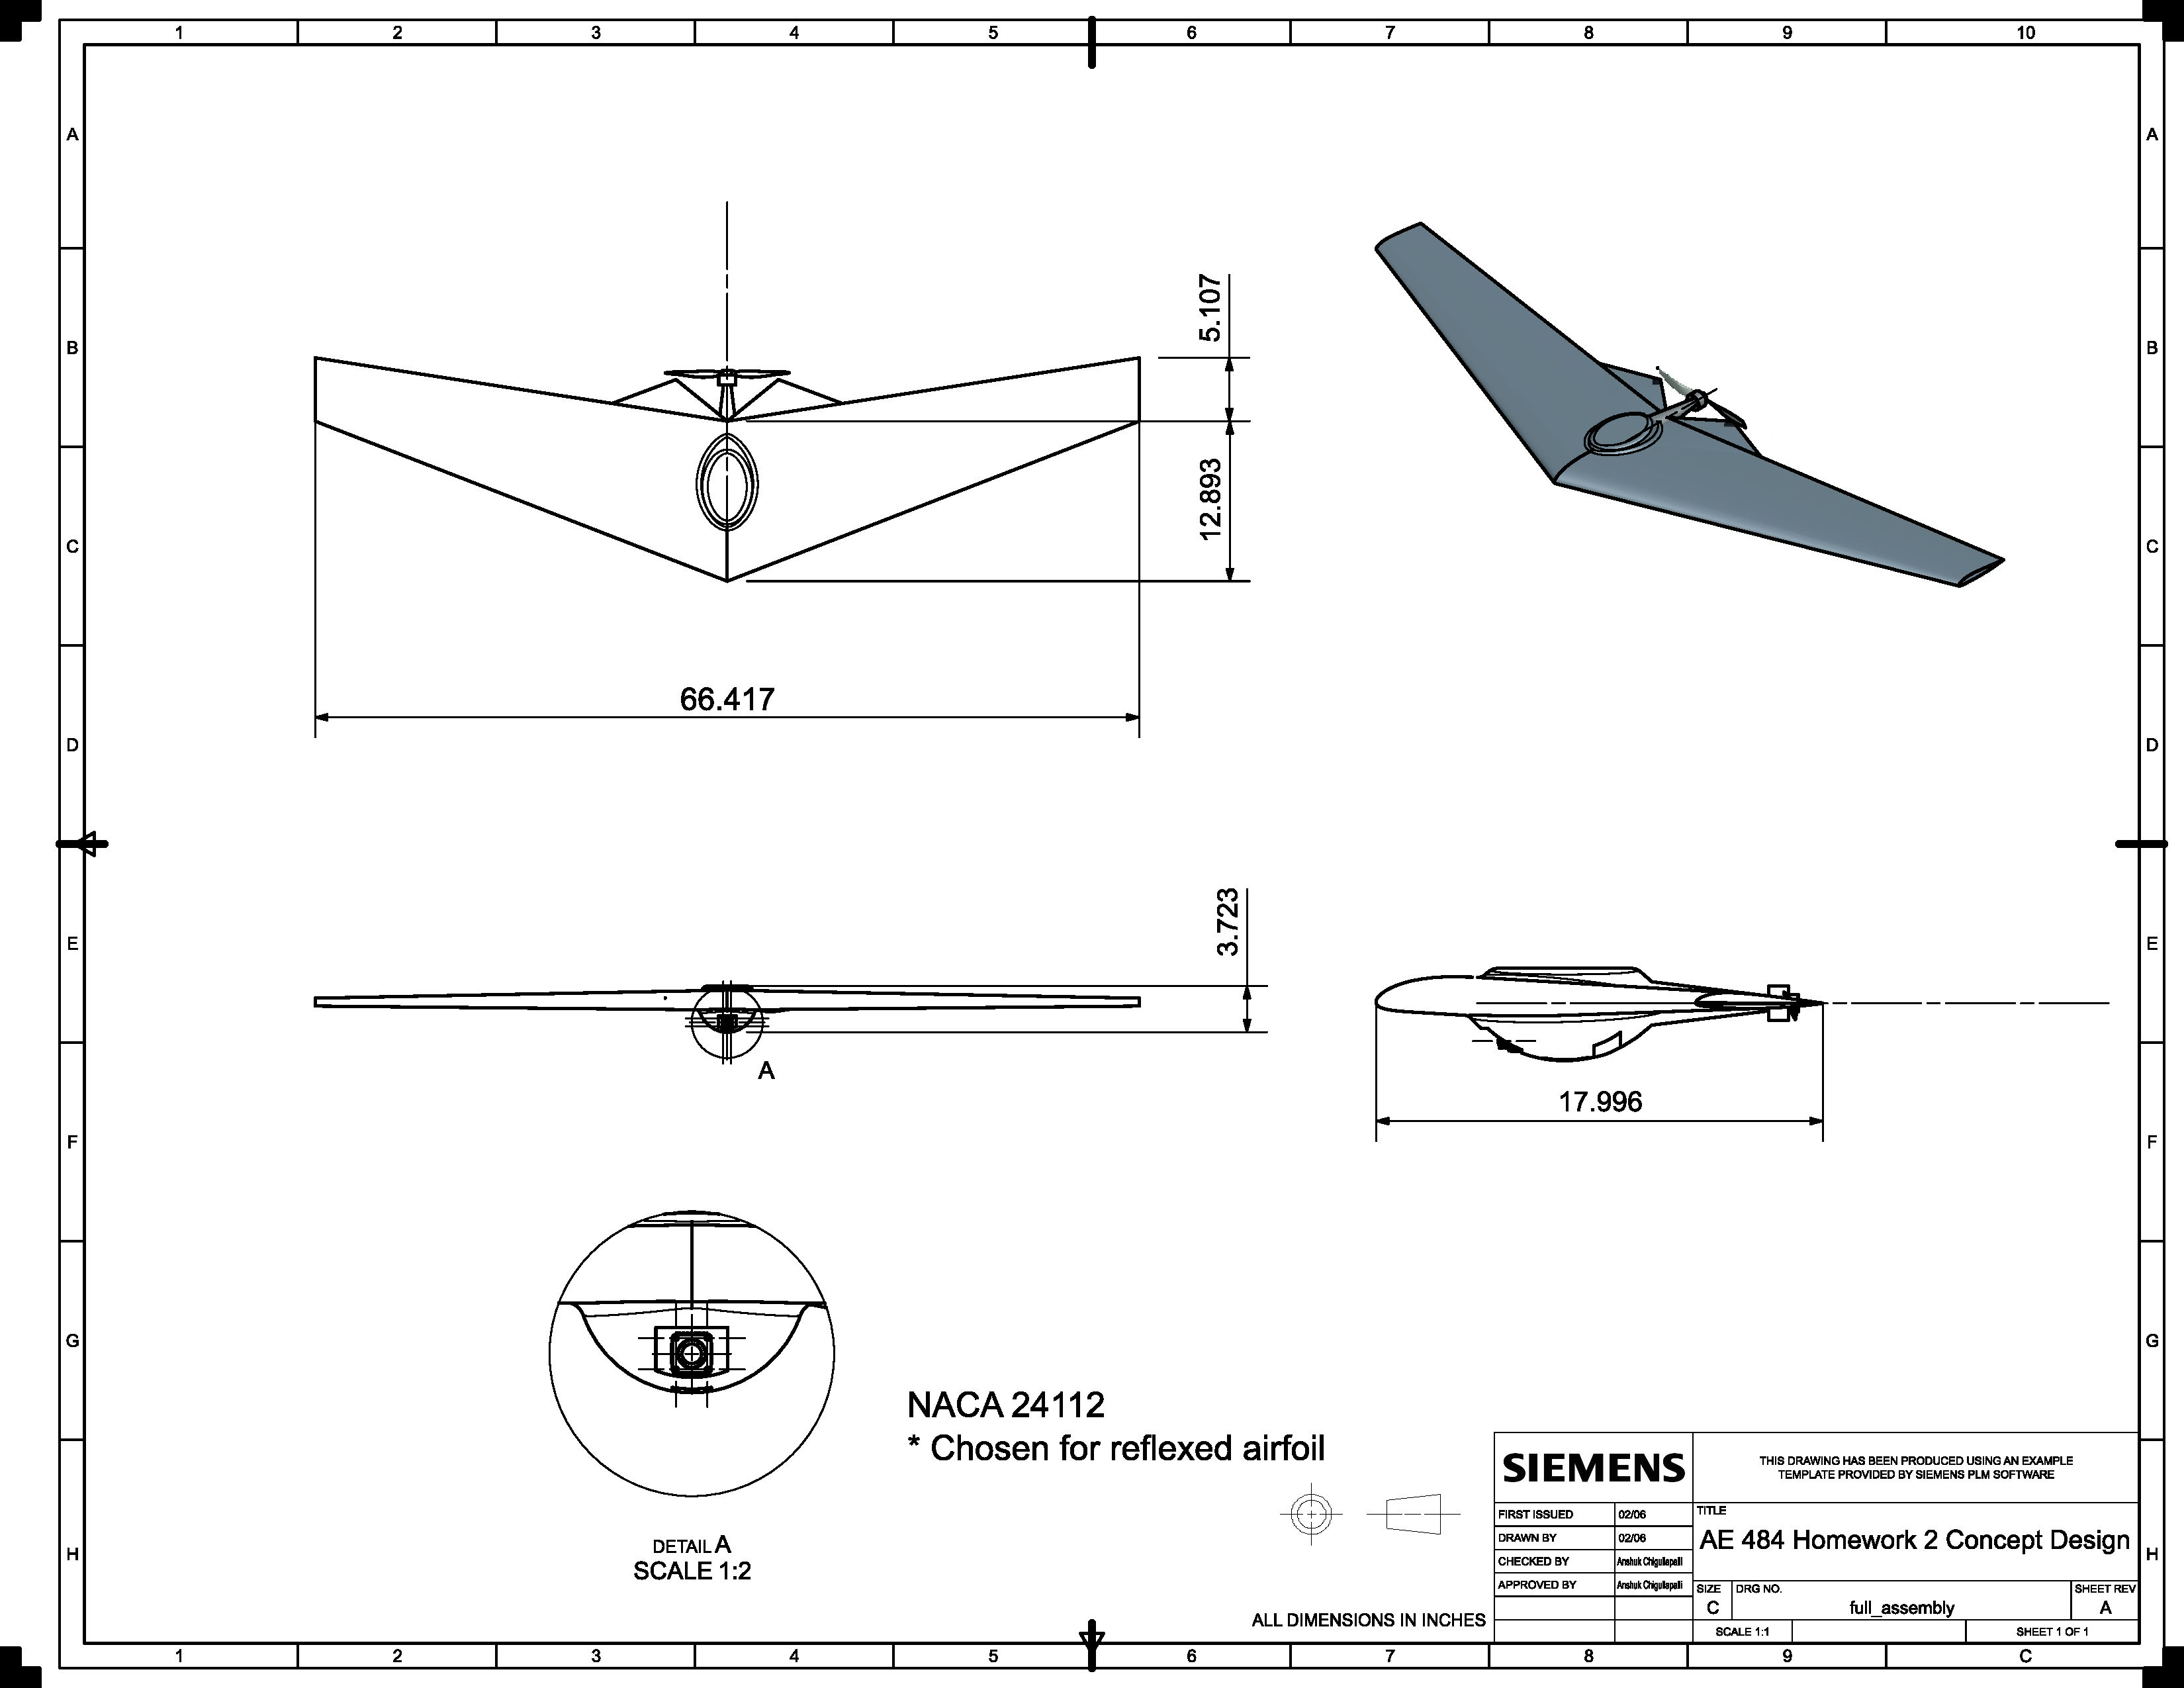
\includepdf[pages=-,angle=90]{../anshuk/HW2_Drawing.pdf}
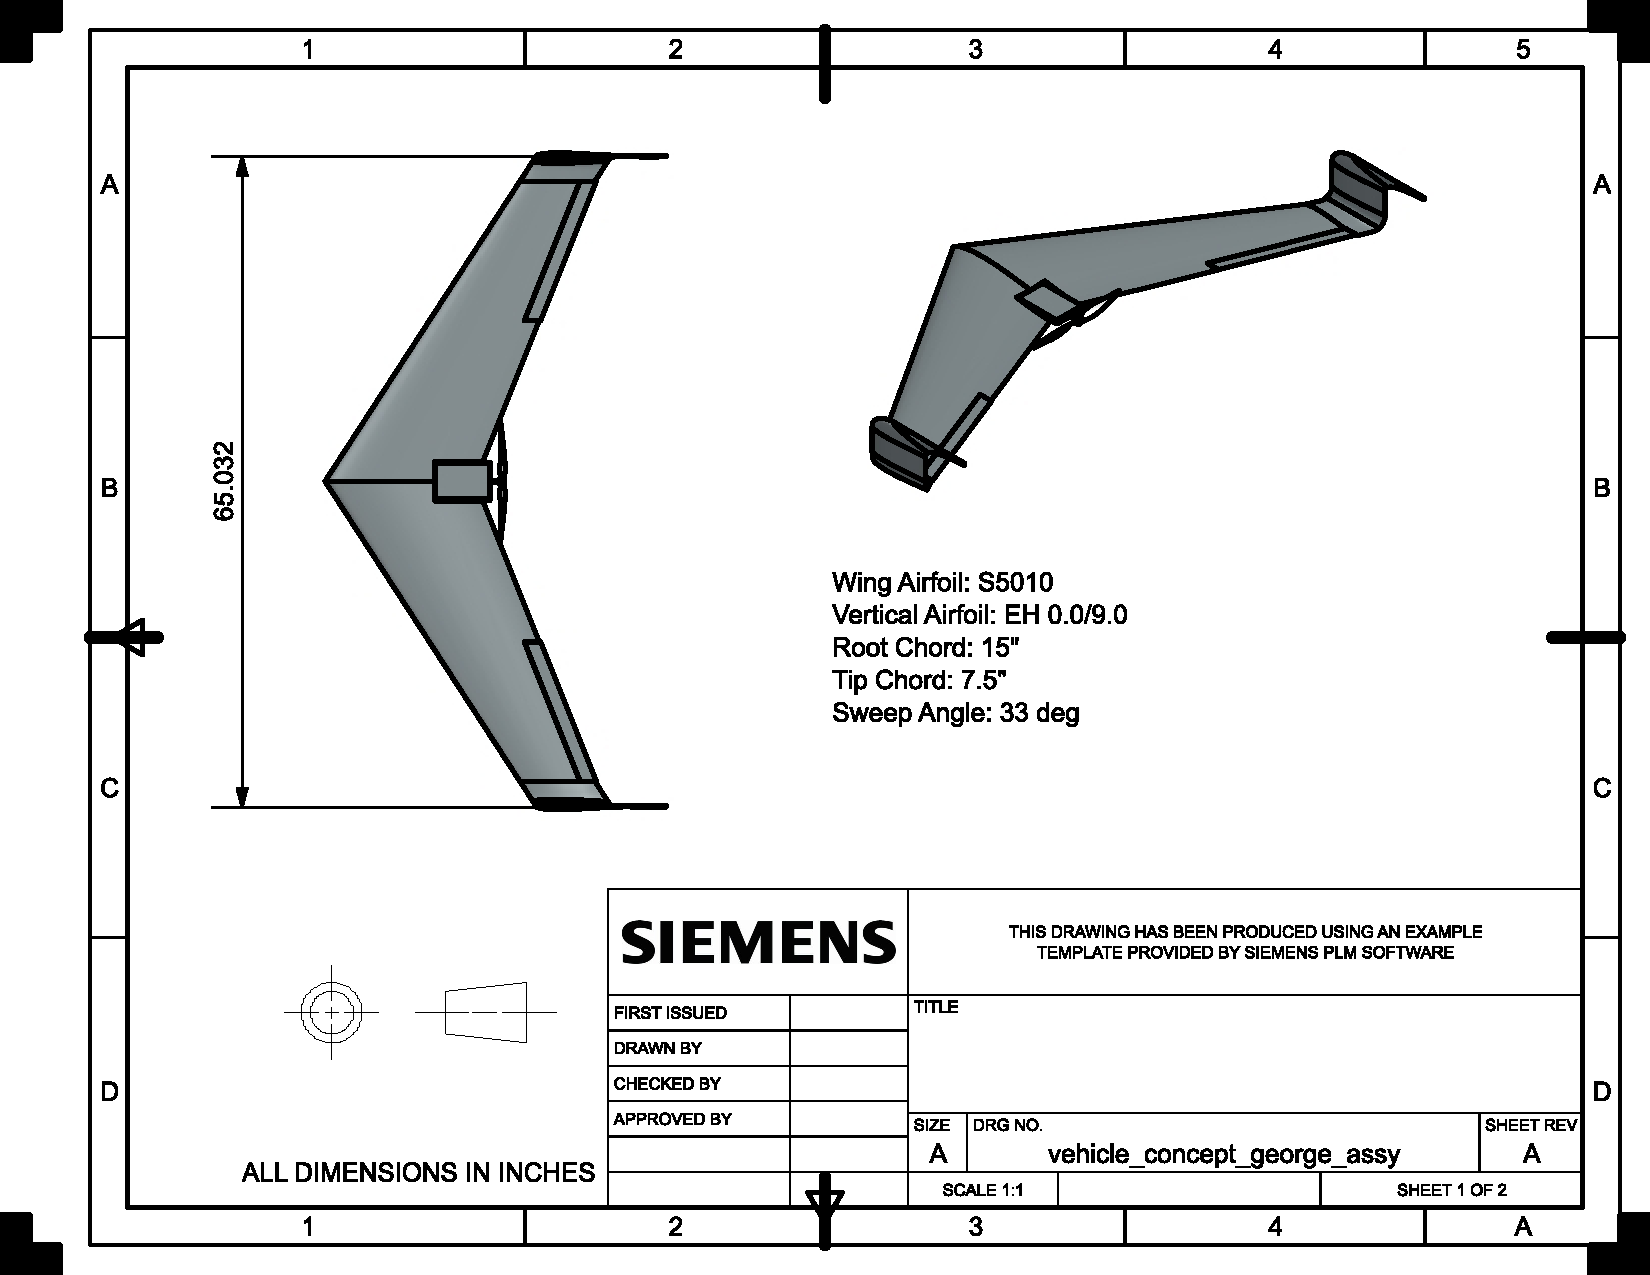
\includepdf[pages=-,angle=90]{../george/Drawings/gpetrov2_vehicle_concept_george_assy.pdf}
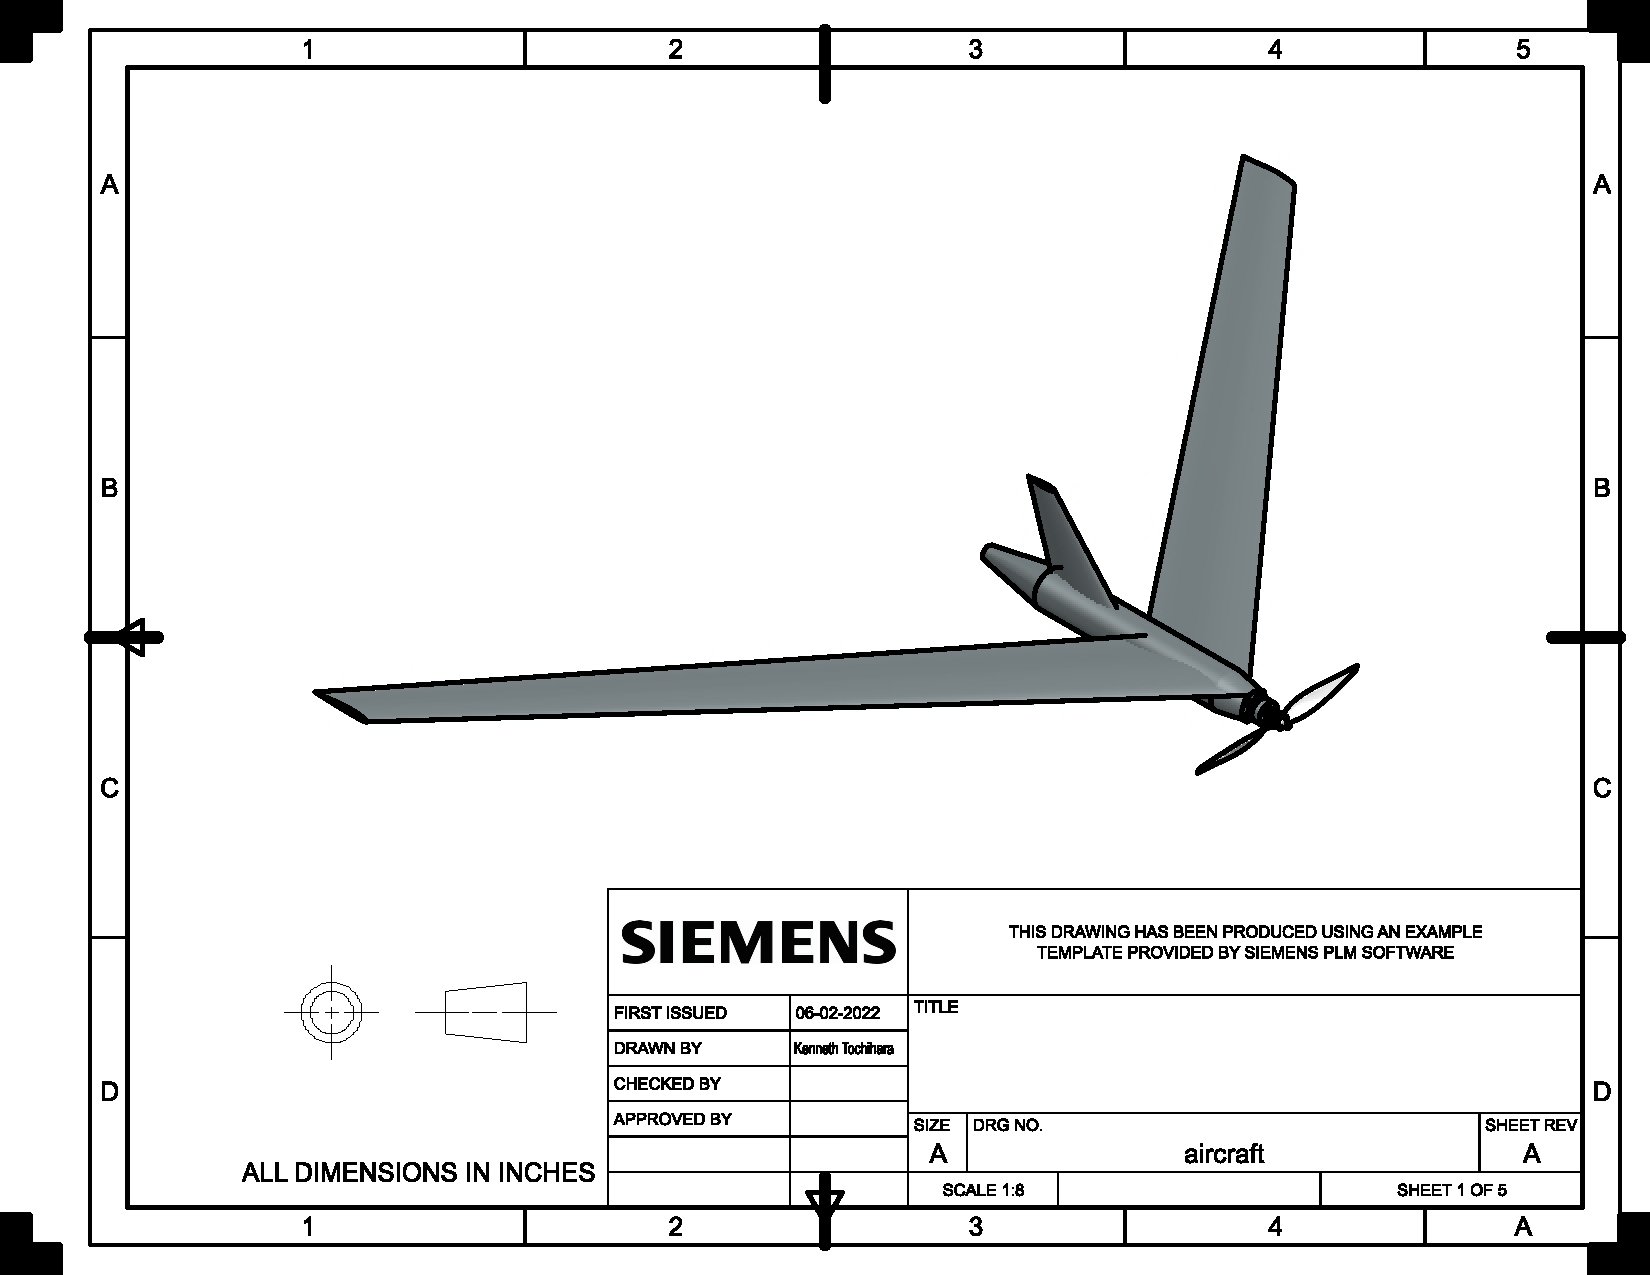
\includepdf[pages=-,angle=90]{../kenneth/ktt3_aircraft.pdf}
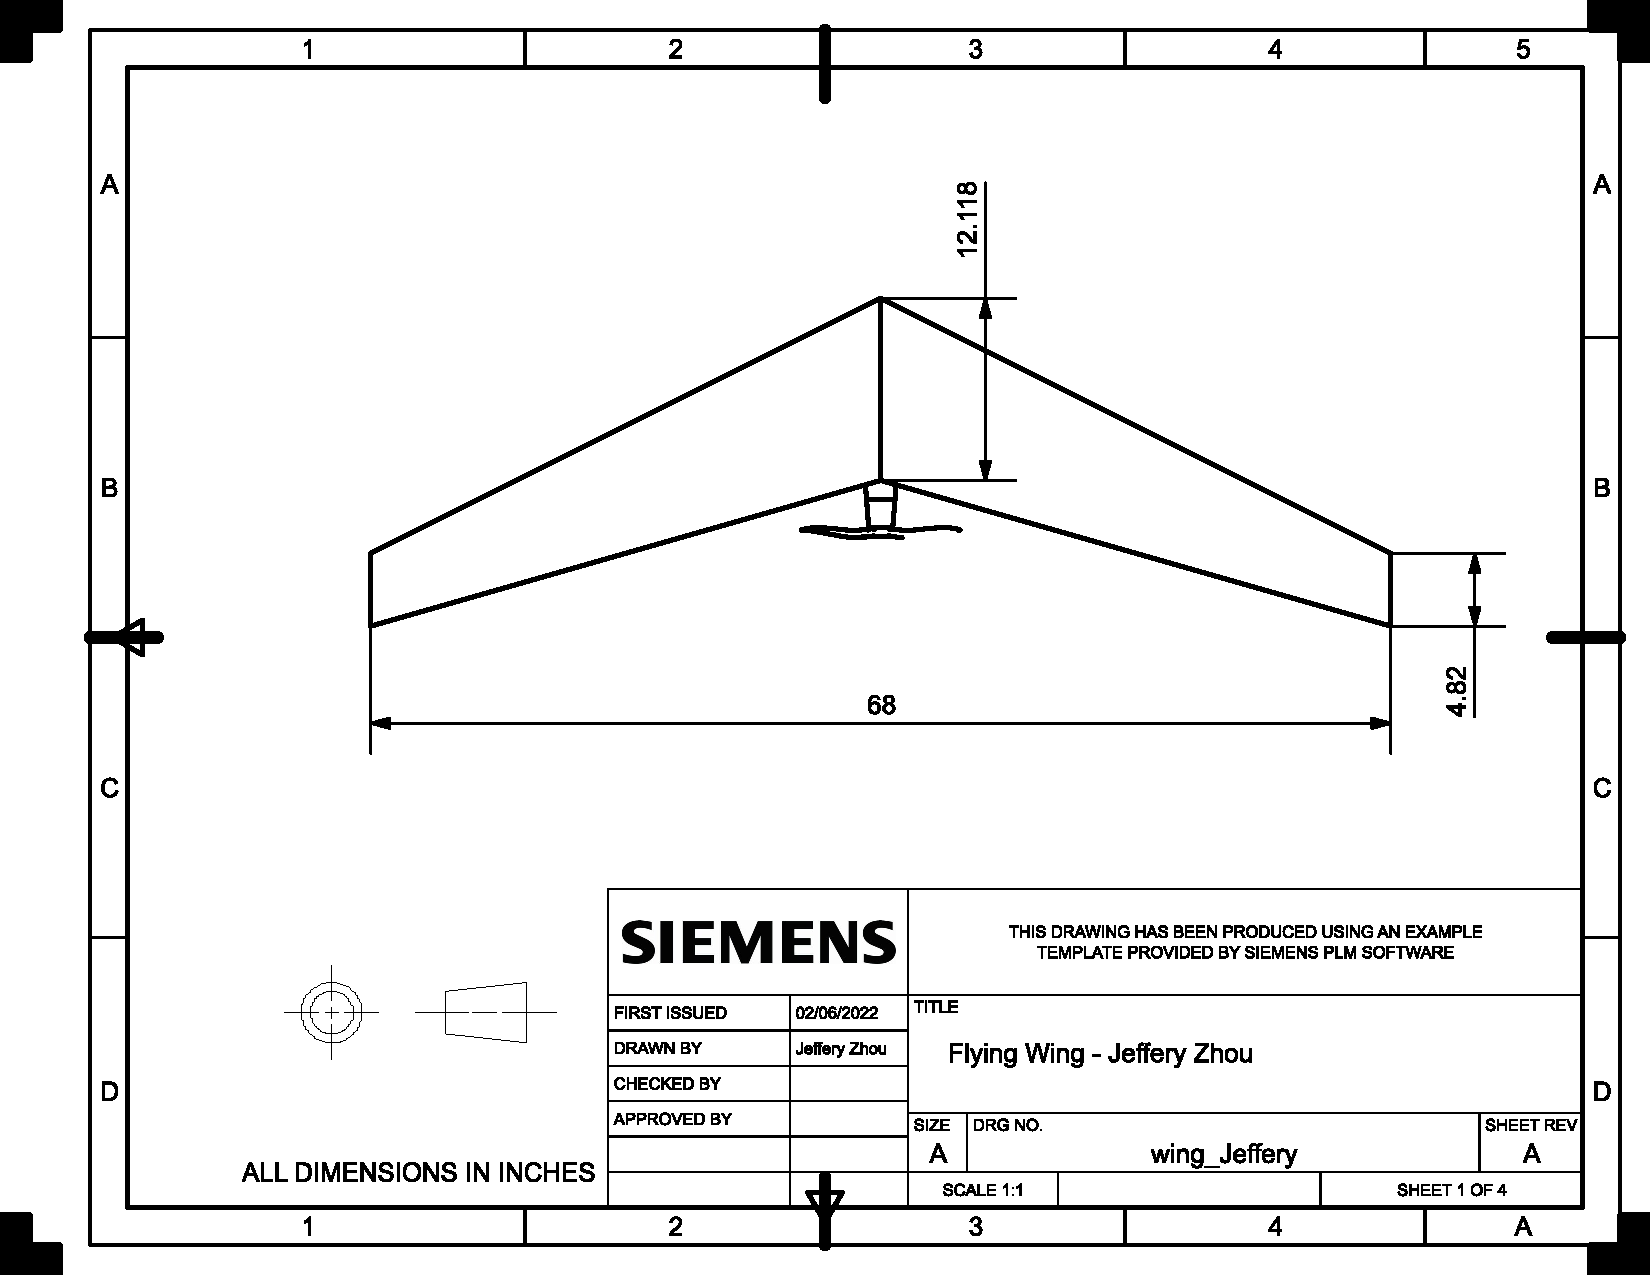
\includepdf[pages=-,angle=90]{../jeffery/shijunz2_wing_Jeffery.pdf}
    
\end{document}